\chapter{Advanced ML Concepts}
\label{chap:AdvancedConcepts}

This chapter extends the capabilities of the subset of the ML language. \myref{sec}{sec:HOF} introduces \emph{higher-order functions} and discusses how they can be compiled securely. Afterwards, \myref{sec}{sec:Functors} explains \emph{functors} and their addition to MiniML. %This chapter continues by showing how the concepts learnt while adding higher-order functions can aid the low-level implementation of functors in \myref{sec}{sec:Functors}.
%The impact of these additions to the language is reviewed.

\section{Higher-Order Functions}
\label{sec:HOF}

A \emph{higher-order function} is a function that allows other functions to be given as input or returns a function as output. \mbox{MiniML} by treats functions as first-class values, meaning that functions represent an entity that can be passed around as a parameter or return value and can be assigned to a variable.

\smallskip
An example of a higher-order function is shown in \myref{lst}{code:LexicalScopingExample}. 
The function \lsttext{addCurried} takes an argument \lsttext{x} and as a result returns another function.
Therefore, \lsttext{addCurried} is a higher-order function.

Since \mbox{MiniML} uses what in literature is known as \emph{lexical scoping}, the function that addCurried returns is allowed access to the non-local or free variable \lsttext{x}, even though it is not defined within the local scope of the function, because its defined scope \emph{lexically surrounds} the definition of the function.

%Since \mbox{MiniML} uses lexical scoping, functions can be defined as shown in \myref{lst}{code:LexicalScopingExample}. The function \lsttext{addCurried} takes an argument \lsttext{x} and as a result returns another function. Therefore, it is a higher-order function. The function \lsttext{innerFunction} has access to the non-local or free variable \lsttext{x}, even though it is not defined in the local scope.

\begin{lstlisting}[frame=single, language=ML,caption={[Lexical Scoping]The use of lexical scoping calls for closures.}, label=code:LexicalScopingExample,numbers=left]
fun addCurried x = 
  let innerFunction y = x + y in innerFunction
\end{lstlisting}

%fun addCurried x = someSPMFunction x
%This is an example of currying.
%Effectively it says:
%fun addCurried x = \y z-> someSPMFunction x y z
%And thus it is owned by the insecure code
%Complex arguments in x are copied when the function is effectively called.
%In the other case, where the secure code creates the closure, complex arguments are already
%copied at the function call of the function creating the closure
%
%It is possible to discern between these two cases. This is no problem (I think).

When a function is created using a call to \lsttext{addCurried} (and possibly saved in a variable to call it later on) this function must be able to access the variable \lsttext{x} that was given as a parameter to \lsttext{addCurried}.
The function entity created and possibly saved in a variable in other words must keep track of the non-local variables it has access to.
This is implemented in \MiniML\ using the concept of \emph{closures}~\cite{Appel}.
A closure consists of a simple function reference together with a list of all the free variables and their values.% called the \emph{referencing environment}.
%a referencing environment which contains all the free variables that are available due to the lexical scoping rules.
%This raises the need to add the concept of \emph{closures} to \mbox{MiniML}.
%A closure consists of a simple function reference together with a referencing environment which contains all the free variables that are available due to the lexical scoping rules.
%When a function is created using a call to \lsttext{addCurried} (and possibly saved in a variable to call it later on) this function must be able to access the variable \lsttext{x} that was given as a parameter to \lsttext{addCurried}.
%The function entity created and possibly saved in a variable in other words must keep track of the non-local variables it has access to.
This list of non-local variables and their values is called the \emph{referencing environment}.

It is possible for these free variables to be complex data such as arrays or abstract data types, for example the Dictionary from \myref{lst}{code:DictionaryStructureExample}. 

Security concerns regarding higher-order functions present themselves in several different ways:

\begin{itemize}
\item The code of the function can be defined within trusted code or untrusted code.
\item When is a closure saved within trusted memory or within untrusted memory?
\item Every free variable of a higher order function can originate from trusted or untrusted code alike.
How do the origin of the free variable and the location of the closure interact?
\item Closures can be passed around as a value, enabling them to cross the security boundary.
\end{itemize}

The compilation scheme presented here requires that the referencing environment are saved in the trusted memory when the closure is created in secure code, and in untrusted memory when it is created in untrusted code.
The creation of a closure happens when a function is used as a value.
For example, \myref{lst}{code:LexicalScopingExample} returns the \lsttext{innerFunction} that it defines as a value.
If \myref{lst}{code:LexicalScopingExample} is located in secure code, its referencing environment and pointer is saved in trusted memory.
If it were located in insecure code, the closure would be located in untrusted code.
The location of a closure in memory defines the security status of a closure: A secure closure is one that is saved in trusted memory.

\label{sec:OnlyLambdaClosures}
For named functions, whose name can be used to pass them as a value, the code where their name is used defines the security status.
For example in \myref{lst}{code:implicit}, the closure that represents the add function is considered to be created by the code of \myref{lst}{code:implicit}, even if this is the insecure context.

This is explained by looking at the unsugared version of this code, as shown in \myref{lst}{code:explicit}.
In this desugared form, it is clear that the code presented in \myref{lst}{code:explicit} creates the closure.
The desugared form finds its justification in examples where the function is already passed one or more of its parameters while leaving the remaining parameters unspecified, a technique called \emph{currying}.
This technique allows for the function insert, defined by the dictionary code of \myref{lst}{code:DictionaryStructureExample}, to be passed as a value with the dictionary into which the key-value pair must be inserted already defined using this code: \lsttext{let closureValue = insert emptyDictionary}.

\begin{lstlisting}[frame=single, language=ML,caption={[Predefined Function Passing]Passing a predefined function.}, label=code:implicit,numbers=left]
foldl (add) emptyList values
\end{lstlisting}

\begin{lstlisting}[frame=single, language=ML,caption={[Predefined Function Passing: Unsugared]Passing a predefined function, unsugared.}, label=code:explicit,numbers=left]
foldl (\x y -> add x y) emptyList values
\end{lstlisting}

Now that the security status of closures had properly been defined and the closure value itself is assigned to trusted or untrusted memory, it is possible to look at the other problems of higher-order function handling, such as the origin of free variables, or the passing of closures across the security boundary.


%Whether or not something is a secure closure is determined by the code that creates the closure.

%Are even the predefined functions represented as closures?

%The origin of free variables of the higher-order function could be trusted or untrusted code alike, just as the function can be defined in either trusted or untrusted code.
%This allows for a case by case analysis of the four distinct combinations of pointer and variable(s).

\subsection{Secure Free Variables For A Secure Closure}

In this case, the code that is executed when the closure is called is located in the secure code section.
The \emph{function pointer} and the \emph{referencing environment} are both in secure memory and are protected from any tampering by the target-level access control model and the checking performed upon compilation.

\subsection{Insecure Free Variables For A Secure Closure}
\label{sec:insecurevaluessecureclosure}
If a closure is created by trusted code with free variables stemming from untrusted code, the values of these free variables should be copied to the referencing environment inside the closure. This is in contrast to the more straightforward low-level solution of having a pointer in the referencing environment to the original value in insecure memory.
This need for copying arises because the low-level code could otherwise change the value of the free variable at any time, as it would be located inside untrusted memory, even mid-execution of the higher-order function.
\myref{lst}{code:CopyFreeVariables} gives an example of two functions that are vulnerable to this kind of attack.

\begin{lstlisting}[frame=single, language=ML,caption={[Copy Free Variables]Changing free variables inside untrusted memory mid-execution can break contextual equivalence.}, label=code:CopyFreeVariables,numbers=left]
fun generateClosure1 freevar =
  let innerFunction x =
    (let b = freevar
    in x + callback 2 + b)
  in innerFunction

fun generateClosure2 freevar = 
  let innerFunction x = x + callback 2 + freevar
  in innerFunction
\end{lstlisting}

The two functions shown in \myref{lst}{code:CopyFreeVariables} are contextually equivalent in \mbox{MiniML}.
Their compiled versions however are not contextually equivalent unless the free variables from untrusted code are copied to the trusted memory.
If no copying of free variables occurs, an attacker could set distinguish a module using \lsttext{generateClosure1} from one using \lsttext{generateClosure2} using the following attack:


\begin{attack}{Call-by-value Attack}
\begin{enumerate}
\item After calling the closure, the attacker forces execution to temporarily be passed back to the unsafe code.
This is achieved in \myref{lst}{code:CopyFreeVariables} by means of the callback function. 
Even when no callbacks are available this type of attack remains possible. For example, in a more powerful language providing a multithreaded environment, this can be forced using a context switch.
\item The context uses the fact that \lsttext{freevar} is saved in unprotected memory to change the value of \lsttext{freevar}. This not possible in the source language, but the target language provides no guarantees against modification of the unprotected memory.
\item If the implementation of \lsttext{generateClosure1} was used, then the result of the closure application depends on when exactly execution was temporarily switched to the attackers context.
If this happened after copying the value of \lsttext{freevar} to \lsttext{b}, which is saved in protected memory, then the result of the closure will not reflect the change of value of \lsttext{freevar} by the attackers context.
If the execution switch happens before this copying of \lsttext{freevar} into protected memory, then the result will be computed using the changed value of \lsttext{freevar}.

In contrast, a version using  \lsttext{generateClosure2} never copies the value of \lsttext{freevar} into protected memory. 
Therefore the result of the closure will allways be computed using the changed value of \lsttext{freevar}.
\end{enumerate}
\end{attack}


The attack described above shows that it is possible to manipulate the low-level versions of the code of \myref{lst}{code:CopyFreeVariables} in such a way that the two different functions do not give the same result. 
Consequently, this means that the contextual equivalence of the compiled code is broken, whereas the source code is unaffected by the attack.
After all, the source language does not allow the memory location of the parameter that was passed to be changed. As a result, step 2 is only possible in the low-level language.

This problem is effectively mitigated by ensuring that upon \emph{application} of the closure every value is copied to the secure environment, conforming to a value-passing call semantic.

However, the \MiniML\ language as described in this work restricts the values that can pass the border between secure code and insecure context to values of either type int or an opaque  type.
Int types are always passed using their effective value.
Opaque types are not susceptible to the attack described above because they can only be manipulated using functions from the structure that declared the opaque type.

%the only values that can pass the border between secure code and insecure context are of an 

%To do: Remark that this is necessary for complex data in regular function calling as well.

%To do: what if the free-variable IS a reference. Then we must follow the reference chain all the way?! No, we follow high-level semantics, and Ref's make MiniML storage aware. ≈If a Reference to storage is created by the attackers context, and this reference is passed as a parameter, it is okay for the attacker to change the value in the storage location, as long as the location remains the same. 

\subsection{Insecure Free Variables For An Insecure Closure}

This combination entails no interaction between the attackers context and the \emph{SPM} beyond the regular means of function calling.
This means that it is not necessary to introduce security measures beyond those discussed in the previous chapters.
How closures and their values are represented is only important to the extent to which implementation for this case and the other cases might be shared by tackling the problem in a generic way.

\subsection{Secure Free Variables For An Insecure Closure}

As stated in \myref{chap}{chap:ACompilationExample}, values originating from secure code should not leave the safety of secure memory provided by the low-level acces control model.
Instead, these values passed must be masked and represented in the insecure code by their masking index.
These same measures are necessary when working with closures.
As long as we obey these measures, and represent secure free variables in the referencing environment by their masking index, they are not susceptible to tampering, illegal disclosure or any other manipulation attacks.
The only way to interact with these secure free variables is by passing them as parameters to functions within the \emph{SPM}.
This shows that the added power of closures does not require any new security measures for this interaction between \emph{SPM} and the attackers context.

%\to do{Should I move this subsection upwards, to right after the discussion of secure closures, or is it more logical to first explain all different free-variable/ closure security status combinations?}
\subsection{Cross-boundary Passing Of A Secure Closure }
Now that it is possible to have a secure closure as a first class value, it can be passed as an object across the boundary between \emph{SPM} and the attackers context.
This section explores the security measures that must be taken when this occurs.
If an \emph{SPM} would pass a closure generated inside its body to the untrusted code, the untrusted code could change the value of the function pointer and inspect or change the values saved in the referencing environment.

Each of these actions break contextual equivalence:
\begin{description}
\item[Change pointer value.] The pointer to the code might be changed to code that makes certain assumptions about the structure used to implement abstract data types.
%For example, if the environment contains 
This way, the context could discern between contextually equivalent \emph{SPM}s in which the assumptions may or may not hold. 
%\to do{provide vulnerability example}
\item[Inspect environment values.]
Assumptions about the way abstract data types are structured can be checked by inspecting the environment values.
%\to do{provide vulnerability example}
\item[Change environment values.] Changing values in the reference environment allows an attacker to discern between a higher order function that first copies its free variables and an equivalent higher order functions that does not, as shown in \myref{lst}{code:CopyFreeVariables}.
\end{description}

As a result, the closure entity itself should not be passed across the boundary between the \emph{SPM} and the trusted code.
Instead, the closure should be masked, just like any value, as explained in \myref{sec}{sec:securityconcerns}. When a closure should be passed to the untrusted code, its corresponding index in the masking map of the \emph{SPM} is passed instead.
%The code pointer inside the closure now points to 
In order to later execute the closure, the \emph{SPM} should offer a \emph{closure-evaluation entry point}.
This entry point first takes a pointer to a closure in the masking map.
Then, because it is located within the \emph{SPM}, the entry point is able to jump to the function pointer specified by the closure and run the function code.

\subsection{The Closure-Evaluation Entry Point}

Because closures can be passed freely, it is possible for insecure code to obtain a closure value.
Of course this insecure code is allowed to make use of the closure, and execute the underlying function.
Execution of a closure is also called the \emph{evaluation} of the closure.
Application of a secure closure by the code in this context is not possible in a direct and straightforward way: the context is not capable of jumping to the code representing the closure because the code that corresponds to the closure might not be located at an entry point of the \emph{SPM} and because it has only knowledge of the masking index of the closure.

To allow insecure code to execute a closure, the \emph{SPM} offers one generic \emph{closure-evaluation entry point}. This entry point should:

\begin{enumerate}
\item Take a masked index as a parameter
\item Allow for an unspecified amount of other parameters to be passed as well, which will be relayed as parameters to the function represented by the closure.
\item Copy the parameters provided by the attackers context in order to prevent \emph{call-by-value attacks} as shown in \myref{lst}{code:CopyFreeVariables}.
\item Look up the masked index and retrieve the closure being referenced, i.e. the function pointer and the referencing environment containing the free variables.
\item Jump to the function pointer providing copies of any parameters it might require, as well as the referencing environment.
\item When execution of the closure is finished, the closure-evaluation entry point provides cleanup of the copied values and performs the tasks necessary for all entry points to the \emph{SPM} code such as register and flag emptying.
\end{enumerate}
%
%The code that implements these different requirements and responsabilities is shown in \myref{lst}{llvm:EvalEntryPoint}.
%
%\begin{lstlisting}[frame=single,numbers=left, language={[x86masm]Assembler}, caption={[Generic Closure Evaluation: Pseudocode]The generic closure-evaluation entry point.},
%label=llvm:EvalEntryPoint]
%fun closureEvalEntryPoint(maskingIndex, spilledParameterPointer)
%    if(! checkIfClosure(maskingMap, maskingIndex)){ //fails if the index does not exist or does not reference a closure.
%        closure = lookUp (maskingIndex) maskingMap //lookUp
%        secureSpilledParameterPointer = copy(spilledParameterPointer)
%        jump (getFunctionPointer(closure))
%        cleanup()
%end 
%\end{lstlisting}

\section{Functors}
\label{sec:Functors}
This section introduces the MiniML concept of functors. Functors can be seen as \emph{functions} from structures to structures.
They accept a structure that conforms to a given signature and create a different structure as a result.

Functors are a way of parametrizing structures.
They can be used to implement a structure that depends on behavior provided by another structure, making only limited assumptions regarding the way this behavior is implemented.
This method of abstraction can be used to create generic data structures.

For example, using functors the dictionary example from \myref{chap}{chap:ACompilationExample} can be made into a more generic data structure. 
The dictionary structure as given in \myref{lst}{code:DictionaryStructureExample} is not type independent since only values of type string are allowed to be used as keys.

Ideally however, how a dictionary works would be described in a generic way that does not care whether the key is of type string, int or any other type.
Instead, it needs only the assurance that some specific functionality is provided by the type.
%This is possible using functors.
%Using functors, it is possible to rewrite the dictionary example in a way that describes how dictionaries work regardless of whether the key is of type string, int, or any other type.
The generic dictionary using functors is shown in \myref{lst}{code:DictionaryFunctor}. 
Its alternative implementation is shown as well in \myref{lst}{code:DictionaryFunctorAlternative}.

\begin{lstlisting}[frame=single,numbers=left, language=ML, caption={[Dictionary Functor Example]A generic dictionary that can take any type of the EQUAL typeclass as its key.},
label=code:DictionaryFunctor, morekeywords={where}]
signature DICTIONARY =
    sig
        type key
        type 'a dictionary
        val emptyDictionary : 'a dictionary
        val insert : 'a dictionary -> key -> 'a -> 'a dictionary
        val lookup : 'a dictionary -> key -> 'a
    end

signature EQUAL =
    sig
        type t
        val equal : t -> t -> bool
    end

structure StringEqual: EQUAL = 
    struct
        type t = string
        fun equal t1 t2  = case String.compare(t1,t2)
                                of EQUAL => true
                                | _ => false
    end
    
functor DictionaryFn (KeyStruct:EQUAL) :> DICTIONARY where type key = KeyStruct.t =
    struct
        type key = KeyStruct.t
        type 'a dictionary = (key * 'a) list
        val emptyDictionary = []
        fun insert d x y = (x,y)::d
        fun lookup |[] x = error
                   |(key,value):ds x = if(KeyStruct.equal key x)
                                     then value
                                     else (lookup ds x)
    end
    
structure StringDict = DictionaryFn(StringEqual);
\end{lstlisting}
%https://www.cs.cmu.edu/~rwh/introsml/modules/subfun.htm
%http://www.cs.cmu.edu/~15150/previous-semesters/2012-spring/resources/lectures/20.pdf
%http://www.disi.unige.it/person/MoggiE/LP/SML/SML-harper/functors.htm
%http://caml.inria.fr/pub/papers/xleroy-applicative_functors-popl95.pdf
%\todo{Edit custom environment so that listings don't pagebreak}

\begin{lstlisting}[frame=single,numbers=left, language=ML, caption={[Alternative Dictionary Functor]The alternative implementations of the dictionary.},
label=code:DictionaryFunctorAlternative, morekeywords={where}, basicstyle=\ttfamily]
functor DictionaryFn(KeyStruct:EQUAL) :> DICTIONARY where type key = KeyStruct.t =
    struct
        type key = KeyStruct.t
        type 'a dictionary = (key list * 'a list)
        val emptyDictionary = ([],[])
        fun insert (a,b) x y = (x::a,y::b)
        fun lookup |[] x = error
                   |(key:ks, value:vs) x = if(KeyStruct.equal key x)
                                         then val
                                         else (lookup (ks,vs) x)
    end
\end{lstlisting}

In order to parametrize over the type of key, the dictionary signature of \myref{lst}{code:SignatureDictionaryExample} was expanded with an extra type named \lsttext{key}, as shown in line 3 of \myref{lst}{code:DictionaryFunctor}.
On top of that, lines 10-14 specify a signature \lsttext{EQUAL} that defines the interface to which a type must comply in order to be a possible key for a dictionary.
Lines 15-21 specify a structure \lsttext{StringEqual} that conforms to the signature needed to act as a key type for a dictionary.

Finally, lines 24-34 show how to define a functor in \MiniML.
First the argument structures and their corresponding signatures are specified, in this case \lsttext{KeyStruct}, whose signature must match signature \lsttext{EQUAL}.
Next, the structure resulting from functor application is bound to the \lsttext{DICTIONARY} signature using opaque ascription.
The choice for opaque ascription ensures that the specific implementation of dictionaries, i.e. as a list of pairs (\myref{lst}{code:DictionaryFunctor}) or a pair of lists (\myref{lst}{code:DictionaryFunctorAlternative}), remains hidden. As a consequence, the dictionary type is an abstract type whose values only can be created by the dictionary structure that results from the functor application.

However, the signature \lsttext{DICTIONARY} hides the implementation of the \lsttext{key} type.
This is a problem, since a user must be able to create values of type \lsttext{key} and pass them to insert function.
The type of values that is put inside the dictionary does not suffer from the same problem as its type is specified parametrically as type variable \lsttext{'a} in the type definition \lsttext{type 'a dictionary}.

This problem can not be solved by specifying the type inside the \lsttext{DICTIONARY} signature, since then it loses the flexibility of allowing multiple different types of keys.
Nor can it be made a type variable in the type definition \lsttext{type 'a dictionary} because type variables are \emph{universally quantified}. 
This means any type can replace them, whereas a dictionary only makes sense if an equality check is possible on the type of its keys.
In other words, specifying the key as a type variable (\lsttext{type ('key, 'a) dictionary}) is unsatisfactory because then the ability to put constraints on the chosen type is lost.

Instead, the problem is solved by modifying our opaque ascription when it is applied to the structure resulting from the functor \lsttext{DictionaryFn}, by specifying that they \lsttext{key} type is equal to the type \lsttext{t} specified in the \lsttext{KeyStruct} that was passed as the functor's argument (Line 24).
This modification makes the type of key freely available, yet still dependent on the specific key structure that was used when the dictionary structure was created using the functor.

The last line of \myref{lst}{code:DictionaryFunctor} shows how the functor \lsttext{DictionaryFn} is eventually applied to the \lsttext{StringEqual} structure, resulting in a dictionary structure saved as \lsttext{StringDict} that uses \lsttext{string} as type for its keys, and compares them using the regular \lsttext{String.compare} function.
This way of specifying a functor allows for very easy change of the \lsttext{key} type, as well as the way that they are compared.
For example, it would require only a minimal change to create a dictionary that disregards capitalization when comparing its \lsttext{key}s of type \lsttext{string}, and it is even possible to cleanly use this alternative implementation in conjunction with the case-sensitive implementation.

\smallskip

\noindent Note that in the example above, the structure \lsttext{StringEqual} was a valid parameter to functor \lsttext{DictionaryFn} because \lsttext{StringEqual}s signature matched to the \lsttext{EQUAL} signature that the functor expected. In the example of \myref{lst}{code:DictionaryFunctor} this is straightforward, the transparent ascription of \lsttext{StringEqual} with signature \lsttext{EQUAL} already assures this.
However, the signature matching relation allows the \emph{candidate} signature to be broader than the \emph{target} signature.
For functor application this means that the argument structure that is passed can define more types or members (values or functions) than the functor expects.
The existence of these types and members however is not assured and the functor can not use them in its body. 
%\to do{mentioned as a prelude to the need of trimming}

\smallskip

As was shown in line 36 of \myref{lst}{code:DictionaryFunctor}, where the \lsttext{DictionaryFn} functor is applied, the addition of functors requires that structures become values, so that they can be passed to functors to create new structures.
However, they are not first-class values: they are bound to names using the special \lsttext{structure} keyword, and can only be returned by functors, not by any \emph{Core} language expression.
As all conditional expressions are part of the \emph{Core} language, structure bindings are always unconditional, which means every structure binding is determined fully before compile time.

\subsection{Security Status of the Resulting Structure}
\label{sec:FunctorSecurityStatus}
Now that functors are added to the MiniML language, it is necessary to determine the security status of functors. 
When is the output structure of a functor considered to be part of the \emph{SPM}, and when is it part of the insecure context?
This question has a simple, yet perhaps surprising answer:
The output structure resulting from a functor has its security status determined by the location of the code defining the functor.

To see why this is the logical choice, consider the example definitions of a dictionary functor in \myref{lst}{code:DictionaryFunctor} and \myref{lst}{code:DictionaryFunctorAlternative}, and the two possible locations for the functor source code:
\begin{description}
\item[In secure code:] 
Suppose \lsttext{DictionaryFn} is defined in secure code, for example when it is part of a library that is offered as a protected module.
This library could choose to implement the \lsttext{DictionaryFn} as in \myref{lst}{code:DictionaryFunctor} (line 24-34) or as in \myref{lst}{code:DictionaryFunctorAlternative}.
Regardless of whether its argument, \lsttext{KeyStruct}, was defined in secure code or in insecure code, the specific implementation of this dictionary is supposed to be abstract.
The resulting dictionary structure is secure.
This means that values of types that are defined by the functor can only be returned to the context as masked values.
In its implementation, the functor can freely call functions of the (possibly insecure) structure, it must however take the same precautions as any callback to insecure code.
%to do: How do we discriminate between structures that are inside the \emph{SPM} and those that are outside the \emph{SPM}? Do we simply check the pointer value against the region? (This is presumably very unsafe).
%to do: How do we represent the structure that was created? It can be used as a parameter for a functor *again*
%to do: Suppose StringEqualCaseSensitive and StringEqualCaseInsensitive are given as argument 
\item[In insecure code:] Suppose \lsttext{DictionaryFn} is defined in insecure code.
Now the choices made when implementing the dictionary are not expected to be abstract. There is no implementation hiding in this case.

This is supported by the consideration that one could replace the functor code with the non-parametrized structure that would result from functor application.
% write out the non-parametrized structure that would result of functor application in MiniML by hand.
This structure would then be a part of insecure code, and of course one would expect that the security status of structures does not change simply due to the use of functors.
\end{description}

A possibly surprising conclusion is that this argument holds, regardless of whether the functor application was done within the secure code or within the insecure code.
As a consequence, application of a functor inside the attackers context can result in the creation of an additional secure structure.

\subsection{Compilation of Functors}
\label{sec:FunctorCompilation}
With the security status of functors determined in \myref{sec}{sec:FunctorSecurityStatus}, %it is possible to think about how to implement functors in the target language.
this section aims to give an overview of the possible methods for implementing functors.
%to do explain
%to do: not by any Core language expression.
%\to do{remark: It is possible to compile away functors (And signatures). See: M. Elsman, Static Interpretation of Modules}

Compilation to the target language has two distinct possibilities of handling structures and functors:
\begin{itemize}
    \item Structures, signatures, functors and functor applications can be compiled away, a technique called \emph{Static Interpretation}.~\cite{Elsman}
    This approach is taken by MLKit\footnote{Available at http://www.elsman.com/mlkit/}.
    As a result, multiple applications of the same functor result in multiple generations of the functor's body, specialized for every combination of parameters.
    \item Structures can be compiled, keeping the members defined by the structures together in the target language in a record like manner called a \emph{frame}.
    Functors can then be compiled using generic code, which receives a reference to the frame representing the structure that is passed as parameter.
    The code of these functors dynamically calls the functions inside the structure received as an argument.
\end{itemize}

The second option is chosen, since it does not duplicate code and is the more standard way of implementing compilation of the Module language of ML.
Also, if functors are compiled away, the code for each resulting structure can only be generated when compiling the functor application.
This would result in either:
\begin{itemize}
\item losing the ability to apply a secure functor outside of secure code
\item having the code representing secure functors outside of secure memory.
\end{itemize}

\smallskip
Choosing the second option means that all members (values or functions) of functors are implemented as stubs that take a pointer to a frame as an additional argument.
%If the functor is located in the secure code segment, the memory locations for all stubs that \emph{do not} correspond to \emph{helper values} are added as \emph{entry points} to the \emph{SPM}.
%This makes them callable by secure and insecure code alike.

The stubs can implement any generic code, and use the information inside the passed frame to call any necessary member defined by the argument structure.

\smallskip

Referencing structures differently in the source and target language raises new security issues when considering functors.
In the source language, structures can simply be referenced by their name.
In the target language however, structures are translated to frames and are referenced by indicating the location of the frame in memory \cmath{loc_{frame}}.

%\smallskip\noindent
%Two main points have to be discussed when considering functors within the context of abstract compilation:
%The first point that needs to be addressed asks what the security status is of the result of functor application.
%Firstly, when is the output structure considered to be part of the \emph{SPM}, and when is it part of the insecure context?
%This is discussed in \myref{sec}{sec:SecurityStatus}.
%The second point, considers 

\myref{sec}{sec:LowLevelRepresentation} expands on the representation and references of structures in the target language, and discusses whether this different representation can be exploited by an attacker.
%discussed in \myref{sec}{sec:LowLevelRepresentation} is whether the representational difference of structures when passing them as an argument to a functor in the high-level language and the low-level language can be exploited to compromise the \emph{SPM} and break contextual equivalence.

\subsection{Target Representation of Structures}
\label{sec:LowLevelRepresentation}
In order to pass structures to functors as an argument, structures are summarized in the target language as a tuple of structure name, and a list of pointers that represent the structure members.
%\todo{Explain the need of trimming, and solve the corresponding trimming problem}.
This target representations are called \emph{frames}.

These frames reside in the memory section corresponding to their security status, for example
structures corresponding to the \emph{SPM} have their frame saved in the protected memory.
This prevents tampering with the frames that correspond to secure structures by the attackers context, such as changing the pointers to the different structure members or changing their order.

\subsubsection{The Structure of Frames \label{sec:StructureOfFrames}}
Structures in MiniML are either defined using the \lsttext{struct} construct or are the result of functor applications to a structure (\myref{fig}{fig:FunctorGrammarExcerpt}).
Both cases must be represented in the target language using frames.

\begin{figure}[htb]
\begin{align*}
\begin{aligned}
\mathit{Structure\ }S ::=\; &\mathit{structure\ } \mathit{id} = \mathit{struct\ }\cdots \mathit{\ end}\\
& |\mathit{structure\ } \mathit{id} = F(S)\\
\\
\mathit{Functor\ }F ::=\;&\mathit{functor\ } \mathit{id} = \mathit{struct\ }\cdots\mathit{\ end}
\end{aligned}
\end{align*}
\caption[\MiniML\ Structure Syntax(excerpt)]{Excerpt from the \MiniML\ syntax related to structures\label{fig:FunctorGrammarExcerpt}.}
\end{figure}

In their most basic form, when defined using the \lsttext{struct} construct, structures are a collection of values and functions.
Frames represent these structures as a combination of structure name and a list of pointers to these values and functions, sorted in alphabetic order.
For example, the frame representation of the \lsttext{StringEqual} structure is shown in \myref{fig}{fig:StringEqualFrame}.
Values or functions inside these structures are now accessible using knowledge of the frame location and the index of the accessed value in the list of pointers.

\begin{figure}[H]
\centering
%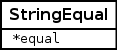
\includegraphics[]{img/StringEqual.png}
\begin{tabular}{|c|}
\hline
StringEqual \\
\hline
*equal \\
\hline
\end{tabular}
\caption[Frame Representation Example: StringEqual]{The frame representation of the \lsttext{StringEqual} structure.\label{fig:StringEqualFrame}}
\end{figure}

To represent functors and the output structure of their application, more information has to be saved. 
For one, functors have an argument, another structure on which it can depend.
To represent the result of a functor application, one needs to track which structure was passed as an argument, i.e. its frame location, as well as the values and functions defined by the functor.
The functor has access to values or functions inside the argument structure using the combination of frame location (\cmath{loc_{frame}}) and the index of the necessary member in the list of pointers inside that frame (\cmath{index_{mem}}).

When accessing these values or functions, the functor can only compute this index based on the members specified in the expected argument signature.
However, as mentioned in \myref{sec}{sec:Functors}, the argument structure can define more members than specified in the argument signature.
Clearly the functor should not access these members.
Yet the index of an expected value or function as computed from the argument signature could be different from the effective index of the corresponding member in the frame.

As a result, the view of the argument structure to the functor must be \emph{trimmed} to that specified the expected signature. 
Because the signature of the argument structure as well as the expected signature are known at compile time, this \emph{trimming} process can be performed at compile time.
The results of this trimming process can be saved in the mapping \cmath{i_{expected} \mapsto i_{effective}}.

Concluding, frames that represent the results of functor applications consist of:
\begin{enumerate}
\item Functor name
\item A pointer to the frame of the argument structure
\item The trimming map
\item The list of pointers to the values and functions, sorted alphabetically.
\end{enumerate}
The frame representing \lsttext{StringDict} from \myref{lst}{code:DictionaryFunctor} is shown in \myref{fig}{fig:StringDictFrame}.

Because the argument structure is represented by a pointer to its corresponding frame, a functor can easily be applied to a structure that already results from functor application.
This allows iterative function application without any additional modifications.

\begin{figure}[htb]
\centering
\begin{tabular}{|c|}
\hline
StringDict \\
\hline
*StringEqual\\
*TrimMap\\
\hline
*emptyDictionary \\
*insert \\ 
*lookup \\
\hline
\end{tabular}
\caption[Frame Representation Example:StringDict]{The frame representation of the \lsttext{StringDict} structure, the output of applying functor \lsttext{DictionaryFn} to structure \lsttext{StringEqual}.\label{fig:StringDictFrame}}
\end{figure}

In order to distinguish frames that represent simple structures from those that represent structures resulting from functor application, the type of frame is tracked using a single bit right at the start of the frame.
For clarity, this value is not shown in the figures representing frames.

\subsection{Creating the Frames}
\label{sec:creatingframes}
\myref{sec}{sec:StructureOfFrames} specified how frames can represent structures.
%\to do{give functors their own chapter? Then 'The Structure of Frames' becomes a subsection with a number}
It also concluded that in order to avoid tampering with the representation of secure frames, secure frames must be located inside the protected memory of the \emph{SPM}.
This section shows that this restriction means not all frames representing structures can be created at compile time (statically), but instead some must be created dynamically.
%prevents the creation of frames at compile time (statically), 
%causes problems with the creation of frames representing structures.

\subsubsection{Problem Example}
When compilation is done within the context of security all secure code is compiled first, and only afterwards is the insecure context compiled.
This \emph{separate compilation} means that the compiled result of secure code is created before compilation of the insecure context starts.

For example, the earlier example of \myref{lst}{code:DictionaryFunctor} could be split up in a secure part and an insecure part as shown in \myref{lst}{code:SecureCodeFragment} and \myref{lst}{code:ContextFragment} respectively.
The code representing the functor is compiled first and separately from the code in \myref{lst}{code:ContextFragment}. 
The \emph{frame} representation for any structures defined inside \myref{lst}{code:SecureCodeFragment} can be created when compiling this file.
However, as \myref{sec}{sec:FunctorSecurityStatus} explains, any structure that results from the application of \lsttext{DictionaryFn} is supposed to be secure as well, meaning their corresponding frames should be saved in secure memory. 
Not all these applications are known when compiling \myref{lst}{code:SecureCodeFragment}.
The application of \lsttext{DictionaryFn} to \lsttext{StringEqual} inside \myref{lst}{code:ContextFragment} results in a new secure structure being created \emph{after} the secure code was compiled.

\begin{lstlisting}[frame=single,numbers=left, language=ML, caption={[Secure Code Fragment]Secure code fragment: secure.ml.},
label=code:SecureCodeFragment, morekeywords={where}]
structure StringEqual: EQUAL = 
    struct
        type t = string
        fun equal t1 t2  = case String.compare(t1,t2)
                                of EQUAL => true
                                | _ => false
    end
    
functor DictionaryFn(KeyStruct:EQUAL) :> DICTIONARY where type key = KeyStruct.t =
    struct
        type key = KeyStruct.t
        type 'a dictionary = (key * 'a) list
        val emptyDictionary = []
        fun insert d x y = (x,y)::d
        fun lookup |[] x = error
                   |(key, value):ds x = if(KeyStruct.equal key x)
                                         then value
                                         else (lookup ds x)
    end
\end{lstlisting}

\begin{lstlisting}[frame=single,numbers=left, language=ML, caption={[Insecure Context Fragment]Fragment of the insecure context: context.ml.}, label={code:ContextFragment}, morekeywords={where}]
...
structure StringDict = DictionaryFn(StringEqual);
\end{lstlisting}

As a consequence, not all frames can be created statically and added to memory at compile time.
Instead they must be added dynamically to preserve the invariant that \emph{all frames representing secure structures are located in secure memory}.
The locations of these dynamically created frames in the \emph{SPM} are kept in a list of frames, called the \emph{f-list}.

\subsubsection{Dynamically Creating Frames\label{sec:DynamicalCreationOfFrames}}
The problem described above only poses itself with functor applications: the binding of secure \lsttext{struct} expressions to a name always happens in secure code.
It's the application of a secure functor, which can happen in insecure code as well, that creates the problem.
How the dynamic creation of frames is handled depends on the location in the source language of the binding of the structure they represent to an identifier.

\begin{description}
\item[Binding in secure code:] When compiling the secure code, it is possible to create frames for all structure bindings inside the secure code, regardless whether they correspond to \lsttext{struct} expressions or functor applications.
Their frames can be added dynamically using preprocessing code located inside the \emph{SPM}. 
Since they are added by code inside the \emph{SPM}, they are guaranteed to be free from tampering.
\item[Binding in insecure code:] The bindings in insecure code require more attention when processing.
When the structure is defined using the \lsttext{struct} expression or the application of an insecure functor, the result will be an insecure structure, whose frame is allowed to be located in insecure memory.
This means that the frame can be added dynamically using preprocessing code inside the attackers context without any further considerations.

When the structure is defined by the application of a secure functor, the result is a secure structure.
This means that the frame must be saved in secure memory.
The output of compilation of the secure code is already created, so the compilation must provide a function that the context can call to create the frame.
This function corresponds nicely with the idea of \lsttext{DictionaryFn(StringEqual)} being a function from structure to structure.

For each secure functor \cmath{Fn}, the compiler adds an entry point to the \emph{SPM} to a function that allows the context to create a frame that would result from applying that functor.
This function expects two arguments: 
\begin{itemize}
\item The index in the f-list that corresponds to the frame that represents the argument of the functor, or the memory location of this frame if the argument is an insecure structure
\item The trimming map that is applied to the structure.
\end{itemize}
Using this information, the function validates its input, creates the frame in secure memory and adds it to the \emph{f-list} before returning.

The validation step is necessary because the preprocessing code is located in insecure memory.
Because this code section is not protected, these preprocessing function calls could be manipulated. 
An attacker could for example apply the functor \cmath{Fn} to a secure argument structure \cmath{S_{a}} that does not match the required signature for functor \cmath{Fn}. 
This would result in the ill-typed output structure \cmath{S_{o}}.

Structure \cmath{S_{a}} can now access members created by \cmath{S_{o}} directly, because both are located in secure code.
By choosing the unsound type assumptions that structure \cmath{S_{a}} makes carefully, this could leak information about the implementation of functor \cmath{Fn}.

Summarizing, when compiling a secure functor the compiler must: %Todo: Nalezen, is dit duidelijk genoeg?
\begin{itemize}
\item Add an entry point in the \emph{SPM}'s metadata corresponding to a function that can create frames representing applications of the functor.
\item Equip this function with the necessary checks to assure that when the argument structure is secure, the arguments signature also matches the expected signature specified by the functor definition.
In other words, code must be added that reads type information about the argument structure and checks it, using \emph{structural typing} as specified in \myref{sec}{sec:StructuralTyping}. This is done to ensure that functor application on secure structures only succeeds if the secure structure signature matches with the target signature.
\end{itemize}

By preserving the order in which functors are applied when adding the frames dynamically, the compiler knows at compilation time the position of every frame in the \emph{SPM}'s \emph{f-list}.
This way, the index in the f-list is a valid substitute for the real location \cmath{loc_{frame}} in memory.
\end{description}

\subsubsection{Implementing Structural Typing Checks}
In order to implement \emph{structural typing checks} when applying secure functors, knowledge about the signatures of structures must be available at runtime.
Because every secure functor has its own dedicated function that creates the frame and performs the necessary type checks, any necessary knowledge about the target signature can be hardcoded.

The signatures of structures within the \emph{SPM} are saved as meta-information linked together with the frame, called the \emph{meta-frame}.
This meta-frame tracks all type definitions and value or function definitions present in the signature.
It needs to formalize a target language representation of types, type definitions and value or function definitions.


The representation of types within the \emph{SPM} is structured as shown in \myref{fig}{fig:TypeRepresentations}.
It consists of representations for the primitive type \cmath{int}, for type variables \cmath{'a}, for types defined in other known structures and for types within the argument structure of a functor.
\begin{itemize}
\item The primitive type \lsttext{int} does not need any additional information for identification.
\item Type variables \lsttext{'a} are denoted only by an index, which says when it was declared. 
This identifies the type variables uniquely, and since type variables are matched with \emph{alpha-equivalence}, their name is not important.
\item Types \lsttext{Struct.t} defined in other known structures \cmath{S} are identified by specifying the location of the corresponding frame \cmath{F_{S}} and its index in this frames type definitions.
\item Types \lsttext{ArgStruct.t} defined in the argument structure of a functor are identified in a analogous way to types \lsttext{Struct.t}. 
They have a different identifier to mark that they depend on the argument structure, and the location of the frame in which they are defined is known only at runtime, so it is not provided.
\end{itemize}
Then, the representation of two composite types is shown, arrays \lsttext{[]} in \myref{fig}{fig:ArrayTypeRepresentation} and pairs \lsttext{(,)} in \myref{fig}{fig:PairTypeRepresentation}.

\begin{figure}[htb]
    \begin{subfigure}[b]{0.20\textwidth}
    \centering
        \begin{tabular}{|c|}
        \hline
        0 \\
        \hline
        \end{tabular}
        \caption{Type \lsttext{int}.\label{fig:IntRepresentation}}
    \end{subfigure}
    \begin{subfigure}[b]{0.20\textwidth}
    \centering
        \begin{tabular}{|l r|}
        \hline
        1 &  \gray \cmath{i_{tyvar}}\\
        \hline
        \end{tabular}
        \caption{Typevar \lsttext{'a}. \label{fig:TypeVarRepresentation}}
    \end{subfigure}
    \begin{subfigure}[b]{0.33\textwidth}
    \centering
        \begin{tabular}{|l c r|}
        \hline
        2 & \gray \cmath{loc_{frame}} & \gray \cmath{index_{type}}\\
        \hline
        \end{tabular}
        \caption{\lsttext{Struct.t}\label{fig:StructTypeRepresentation}}
    \end{subfigure}
    \begin{subfigure}[b]{0.25\textwidth}
    \centering
        \begin{tabular}{|l r|}
        \hline
        3 & \gray \cmath{index_{type}}\\
        \hline
        \end{tabular}
        \caption{\lsttext{ArgStruct.t_{i}}\label{fig:ArgTypeRepresentation}}
    \end{subfigure}
    \\
    \\
    \begin{subfigure}{0.50\textwidth}
    \centering
        \begin{tabular}{|l r|}
        \hline
        4 & \gray \cmath{type}\\
        \hline
        \end{tabular}
        \caption{Type \lsttext{[]}.\label{fig:ArrayTypeRepresentation}}
    \end{subfigure}
    \begin{subfigure}{0.50\textwidth}
    \centering
        \begin{tabular}{|l c r|}
        \hline
        5 & \gray \cmath{left_{type}} & \gray \cmath{right_{type}}\\
        \hline
        \end{tabular}
        \caption{Type \lsttext{(,)}.\label{fig:PairTypeRepresentation}}
    \end{subfigure}


    \caption[Type Representations For Metaframes]{This figure shows the representation of all different types \label{fig:TypeRepresentations}}
\end{figure}

\begin{figure}[htb]
\begin{subfigure}[b]{\textwidth}
    \centering
    \begin{tabular}{|l c c c r|}
    \hline
    name & \cmath{i_{typevar}} & \cmath{\#_{typevar}} & implementation & opacity\\
    \hline
    \end{tabular}
    \caption{Type Definition\label{fig:TypeDefinitionsRepresentation}}
\end{subfigure}
\\
\\
\begin{subfigure}[b]{\textwidth}
\centering
\begin{tabular}{|l r|}
    \hline
    name & implementation\\
    \hline
    \end{tabular}
    \caption{Value Definition\label{fig:ValueDefinitionsRepresentation}}
\end{subfigure}
\caption[Metaframe Elements]{The representation of type \textbf{(a)} and member definitions \textbf{(b)}.}
\end{figure}

The representation of type definitions is shown in \myref{fig}{fig:TypeDefinitionsRepresentation}, and that of member definitions in \myref{fig}{fig:ValueDefinitionsRepresentation}.

For the signature of an argument frame to match the target-signature, every type definition in the target signature and every member must have a match in the meta-frame, as explained in \myref{sec}{sec:StructuralTyping}:

\begin{description}
\item[Matching type definitions]
First, a match is searched for all type definitions within the target signature:
Searching inside the meta-information for a matching type definition can be done by scanning the meta-information for a type definition with the same name.
If no type definition with the same name is available, the two signatures do \emph{not} match.

If such a type definition is available, check the number of type variables \cmath{\#_{typevar}} it expects.
If the type definition in \emph{target} and \emph{candidate} signature take a different number of type variables, the two signatures do \emph{not} match.

If the matching type definitions take the same number of type variables, then the opacity of the type definition in the \emph{target} signature is of importance. If the type is \emph{not} defined opaque, the implementation of the two matching type definition is matched to ensure the same implementation.
\item[Matching members]
Next, for all value or function definitions inside the \emph{target} signature, a matching definition inside the \emph{candidate} signature is identified using the names.
In this matching, only the members which correspond to a result of the \emph{trimming map} are considered.

When a name match is found, its type is checked.
When creating a meta-frame, any type used in the typing of members is substituted by its implementation until the first opaque type is encountered.
This ensures that checking whether the type of two members match can be done by checking that either the type stated in the candidate signature is exactly the same as the type in the target signature, or it is a type variable that substitutes \emph{consistently} for the type listed in the target signature.
\end{description}

\subsubsection{Creating Meta-Frames}
Implementing \emph{structural typing} required knowledge about the signatures of structures to be available at runtime.
It introduced \emph{meta-frame}s as a type of meta-information linked together in memory with the frame.
These \emph{meta-frame}s track all type definitions and member (value or function) definitions present in the structures signature.

The content of these \emph{meta-frame}s can mostly be determined at compile time. This surely is the case for structures, but it also is the case for functors that are not modified by a \lsttext{where} expression.
This means that the function that creates a frame corresponding to a functor application can largely hardcode the content of the corresponding meta-frame.
When creating a meta-frame, any type used in the typing of a member is substituted by its implementation until it contains only opaque types, counting \lsttext{int} as an opaque type.

\begin{description}
\item[Handling where Expressions] 
Only \lsttext{where} expressions of the template \lsttext{where type t = ArgStruct.t'} can not be processed at compile time.
For these expressions, a compiler must produce the structural typing checks so that they check:%Todo: Nalezen, is dit duidelijk genoeg?
\begin{enumerate}
\item That the implementation of type \lsttext{t} is in fact \lsttext{ArgStruct.t}.
\item What the opaqueness and implementation of type \lsttext{ArgStruct.t} is, so that any reference to type \lsttext{t} or \lsttext{ArguStruct.t} can be substituted by its implementation.
\end{enumerate}
\end{description}
\subsection{Calling Structure Members}
Access to any member of a source language structure (i.e. one of its values or functions) is uniquely determined in the target language using the location (\cmath{loc_{frame}}) of the frame in memory and the index of the member (\cmath{index_{mem}}) in its list of pointers.

In the source language, all members are either accessible across the security boundary or strictly accessible only within the same structure, so the same must hold for the target language.
It is easy to make members accessible only from within the same structure: they are not given an entry within the list of member pointers, and their location is not made into an entry point for the \emph{SPM}.

All other members are accessible across the security boundary. However, as frames are saved in the memory corresponding to its security status, the attackers context is not able to access frames corresponding to structures within the \emph{SPM} directly.
Worse, the attackers context is not even allowed to know the exact location \cmath{loc_{frame}} of these secure frames.

%To solve this, all $loc_{frame}$ are masked by inserting them into a list of frames, called the \emph{f-list}, in the order of their definitions.
This is solved by inserting all \cmath{loc_{frame}} into the \emph{SPM}'s list of frames (\emph{f-list}) that was introduced in \myref{sec}{sec:DynamicalCreationOfFrames}. 

Frames that were created in secure code are sorted alphabetically by the identifier they were bound to and put in the \emph{f-list} first.
This alphabetical ordering is necessary because changing the order of structure bindings does not break contextual equivalence at the high-level \MiniML\ language.
The frame locations of frames created in insecure code are appended in the order of their definitions.
This means that the specific mapping of an identifier to the value of its index is known statically.

%\to do{Sort those bound in secure memory alphabetically, and append those bound to an identifier in insecure context in the order of their definition! Otherwise, contextual equivalence is broken, isn't it?}
%TO DO: Doesn't this break contextual equivalence? Solution: Sort alphabetically for those created in secure memory!
Anywhere a secure structure is used in the source language, it is represented in the target language by the \cmath{loc_{frame}} pointer or its masking index in the \emph{f-list}.

To allow context code to access members from secure structures, a getter function is provided that is located inside the \emph{SPM}.
This getter function corresponds to an \emph{entry point} to the \emph{SPM}.
The context can now pass an index in the \emph{f-list} \cmath{index_{f-list}} and an index for the structure member \cmath{index_{mem}}, as well as any arguments that should to be passed to the member to this getter function.
%to do: alternatively the pointer to the value is passed directly
This getter, because it is located in secure code, can access the \emph{f-list} and the frames themselves.
It then does the following things:
\begin{itemize}
\item Check whether \cmath{index_{f-list}} corresponds to a real frame by using the expected length of the list.
Since structures resulting from a functor application are added dynamically, a situation could arise where the corresponding frame has not yet been added, or where something went wrong while adding the frame.
In this case the getter function must not allow the \cmath{index_{f-list}} to be used.
\item Use \cmath{index_{f-list}} to get a \cmath{loc_{frame}} for the correct frame.
\item Check whether the frame represents a simple structure or the result of functor application.
\item Look up \cmath{index_{mem}} in the list of pointers within the frame to get a pointer to the accessed member.
\item Call this member with any relevant arguments.
In case the frame represents the result of functor application, the pointer to the frame must be provided as a parameter when calling the member.
The function implementing the member will uses this frame to determine the argument frame.
%argument frame must be provided when calling the value.
%By design, a pointer to this frame is always present within the frame representing the functor output itself.
\item Return any results to the caller.
\end{itemize}

The getter functions only as an additional level of indirection, so it presumes that any clearing of flags, registers, masking of values or other precautionary measures have already been taken care of by the functions that it passes the call to.

Since all structure values are accessible through this getter function, the separate structure value stubs do \emph{not} have to be entry points in the \emph{SPM}. The getter function will always be necessary, because insecure functors that call a member in their argument structure can not hardwire a specific entry point in their generic code.
\\[1em]
\label{sec:StaticDefinitionFunctorApplication}
Indeed, the stubs corresponding to structure members \emph{cannot} be made entry points in the \emph{SPM}, because the source language context is oblivious to whether a structure bound in secure code was the result of a functor application, or was statically defined. This corresponds to \myref{lst}{lst:FunctorApplicationOrStaticDefinition1} being contextually equivalent to \myref{lst}{lst:FunctorApplicationOrStaticDefinition2}.

\begin{lstlisting}[frame=single,numbers=left, language=ML, caption={[Functor Application or Static Definition: 1]Binding StrA and StrB using functor application.},
label=lst:FunctorApplicationOrStaticDefinition1, morekeywords={where}]
functor F(ArgStruct:ArgSig) :> OutputSig =
    struct
        val x = ArgStruct.f x
    end
    
structure StrA = F(Arg1)
structure StrB = F(Arg2)
\end{lstlisting}

\begin{lstlisting}[frame=single,numbers=left, language=ML, caption={[Functor Application or Static Definition: 2]Binding StrA and StrB using both static definition and functor application.},
label=lst:FunctorApplicationOrStaticDefinition2, morekeywords={where}]
functor F(ArgStruct:ArgSig) :> OutputSig =
    struct
        val x = ArgStruct.f x
    end
    
structure StrA :> OutputSig =
    struct
        val x = Arg1.f x
    end

structure StrB = F(Arg2)
\end{lstlisting}


If stubs were made entry points in the target language, the difference between static definition and function application would break contextual equivalence.
\begin{itemize}
\item Compiling \myref{lst}{lst:FunctorApplicationOrStaticDefinition1} means calling value \lsttext{StrA.x} would use the same entry point as calling \lsttext{StrB.x}.
\item Compiling \myref{lst}{lst:FunctorApplicationOrStaticDefinition2} means calling value \lsttext{StrA.x} would use an entry point different from the one used when calling \lsttext{StrB.x}
\end{itemize}
Clearly, this would result in \myref{lst}{lst:FunctorApplicationOrStaticDefinition1} and \myref{lst}{lst:FunctorApplicationOrStaticDefinition2} not being contextually equivalent in the target language.
\\[1em]
The addition of a generic getter function that is used to access any value or function defined on a structure adds an additional level of indirection in calls between the insecure context and the secure code.

To illustrate this, \myref{fig}{fig:callstackcomparisonsimple} shows the flow of execution corresponding to a function call in the simple \MiniML\ language or the work of Agten et al.~\cite{Agten:2012:SCM:2354412.2355247}. As a comparison, \myref{fig}{fig:callstackcomparisonadvanced} shows the flow of execution for that same call in the \MiniML\ language with advanced concepts.

\begin{figure}[htb]
\centering
\begin{subfigure}{\textwidth}
\centering
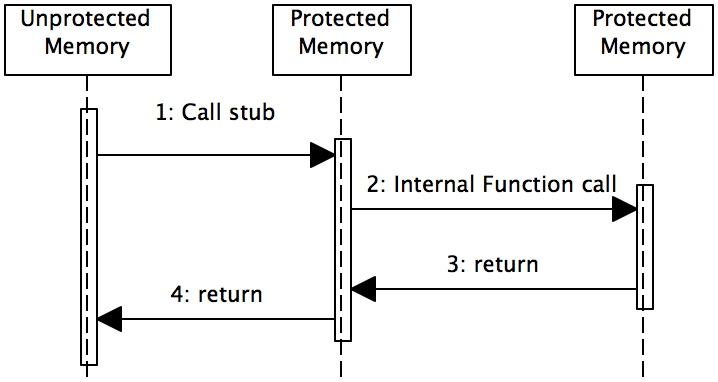
\includegraphics[scale=0.6]{img/Simple.png}
\caption{Execution flow in the simple \MiniML\ language. \label{fig:callstackcomparisonsimple}}
\end{subfigure}
\\
\begin{subfigure}{\textwidth}
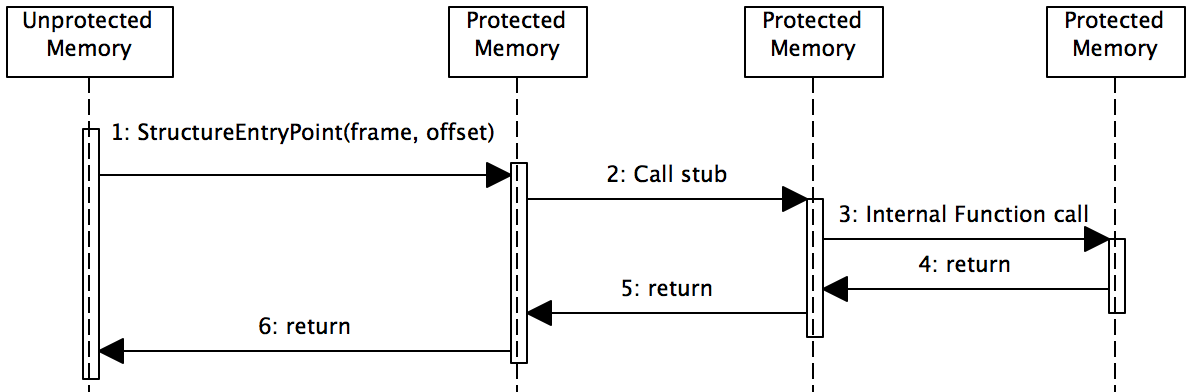
\includegraphics[scale=0.6]{img/Advanced.png}
\caption{Execution flow in the \MiniML\ language. \label{fig:callstackcomparisonadvanced}}
\end{subfigure}
\caption{Comparison of execution}
\end{figure}
%However, in order to allow optimization, the structure values could safely be made entry points of the \emph{SPM} with only minimal changes to the scheme above:
%\begin{itemize}
%\item The high-level language context is oblivious to whether a structure bound in secure code is the result of functor application or was statically defined.
%As a result, when the stubs that access a structure value are made entry points to the \emph{SPM}, all stubs must take a frame location as an extra argument.

%\item When all stubs must take a frame location as an extra argument, the frame location can no longer be that of the argument structure because statically defined structures do not have an argument structure. Instead, the passed frame location must be the location of the \emph{own} frame.
%When the stub represents a value of a functor, 
%\end{itemize}

%The values within a structure resulting from functor application are stubs that expect an extra argument, the location of the \emph{own} frame.
%If these stubs can be called directly by the context without the getter function, care must be taken to check that the location of the own frame is either inside insecure memory or is interpreted as a mask in the f-table.

%When providing this optimization, structures that were defined statically, i.e. \emph{not} as a result of functor application, need to take the location of their extra argument 


% is able to read the pointer corresponding to the $(loc_{frame}, index_{mem})$ pair and call the necessary value.
%It can then return any results to its caller.

%If the values are inside a structure resulting from functor application, care has to be taken.
%The code representing the values expects the frame of the argument structure to be passed as a first argument.
%By design, a pointer to this frame is always present within the frame representing the functor output itself.
\subsection{Security Consequences}

In order to explore the possibility of contextual equivalence breaking due to the representation of structures differing between source and target language, the possible combinations of functor and structure security and the relevant security measures are recapped here case by case.
%Since functor application results in a structure as well, these structures must also be representable as frames.
%In order to allow this, frames consist of a type indicator that identifies it as a structure defined using the struct keyword, or a structure resulting from functor application.

%to do: Trimming problem, problem with iterated functor applying. (When applying a secure functor, the resulting structure must be saved in the list of structures in secure memory. This consists of a pointer to the functor
%to do: suppose functor application is done in the insecure code. Structure is in secure code. Regardless of where the functor is located, the linker knows what signature it expects and can trim down the 
%Origin problem: What is the origin of the structure. Is it a pointer in the insecure memory, or is it a masking index?
%Fresh type names at every application, even to the same arguments! http://books.google.be/books?id=oPaAAahVu_kC&pg=PA345&lpg=PA345&dq=functors+sml+each+new+application+provides+fresh+types&source=bl&ots=g-VRLSeChc&sig=v4t4Ch42F-pktGaLpqgMq51K92k&hl=en&sa=X&ei=YvfGU92vHYrR7Aa89oGoDw&ved=0CCsQ6AEwAQ#v=onepage&q=functors%20sml%20each%20new%20application%20provides%20fresh%20types&f=false
%note whether the application was really performed!
\begin{description}
\item[Secure functor and secure structure] 
%In this case, at the moment of functor application a new frame is created representing the result of this functor application. This consists of 
The \emph{frame} representing a structure is located in the same part of memory as the structure was defined.
Since in this combination both the functor code and the frame are located inside protected memory, no tampering is possible.
When functor code is called with a reference to the frame in secure memory, the functor code is able to read the frame directly, because the functor is part of the \emph{SPM}. It can then call any member of the argument structure using the pointer provided by the frame.

If the application of the secure functor is done inside insecure code, the frame creating function corresponding to this functor must be called, and the types are checked dynamically using type information in the \emph{meta-frame}.
\item[Secure functor with insecure structure]
When a secure functor is applied to an insecure structure, its result is a secure structure that calls functions provided by the insecure structure.
The resulting structure \emph{depends} on the insecure structure.
It must call these functions using the same precautions as regular callbacks to the attacker's context.
Of course the pointers that represent these functions can be manipulated by the attacker because the frame is now located in insecure memory.
However, because contextually equivalent implementations of the functor must perform the same callbacks with the same arguments in the source language in the same order, their target language versions will always use the same pointers provided by the insecure frame, with the same parameters in the same order.
As a result, the regular precautions, such as clearing registers, switching the stack and masking values that pass from secure code to the insecure context, are sufficient to ensure preservation of contextual equivalence of the functors in the target language. 

Additionaly, when calling the code in insecure context, the real return address should be saved in secure memory, and the return address entry in the insecure stack should be modified to point to the returnback entry point~\cite{Agten:2012:SCM:2354412.2355247}.
This returnback entry point is listed in the entry points of the \emph{SPM}.
The returnback entry point retrieves the last real return address saved in memory, and jumps to this address.

If the application of the secure functor is done inside insecure code, the frame creating function corresponding to this functor must be called, and the types are checked dynamically using type information in the \emph{meta-frame}.
%to do: OR depends on values
\item[Insecure functor with insecure structure]
In this case, both the functor code and the frame are located inside unprotected memory.
The structure that results from the application is considered to be part of the attacker's context.
The use of members from the insecure structure by code inside the insecure functor can happen without any security precautions, as the expected behavior is simply equivalent to that of an unparametrized structure in the attacker's context that depends on another structure of this same context.
\item[Insecure functor with secure structure]
Because the code of the functor is now located outside of the \emph{SPM}, special care needs to be taken when the functor depends on members of the structure.
Because the frame \cmath{Fr_{s}} representing the structure is now in secure memory, the functor cannot manipulate this frame or perform reads on this frame.
In order for insecure functors to call these functions, an entry point is provided by the \emph{SPM}, corresponding to a generic getter that takes as argument a \cmath{loc_{frame}} and an \cmath{index_{mem}}, as well as any arguments that would otherwise be passed directly.
As a result, the generic getter returns the result of the call to its caller.
%to do: possible variant: this generic entry point returns a pointer
%As a result, a pointer to the correct entry point is returned to the insecure code, which it can then call with the necessary arguments.
%todo
\end{description}

%\to do{When calling values of the argument structure, the functor must at all times take care to determine whether the argument frame represents another functor output, or a basic structure, since calling a value within functor output requires the first argument to be a frame pointer to the argument structure. Should I add this remark in text, or should I provide code that does this check, and refer to that.}

\section{Conclusion}
In this chapter, some more advanced concepts of ML were added to the \MiniML\ language: higher-order functions and functors.

Higher order functions, and the closely related concept of closures, can be introduced if certain sensitive information, such as environment values and pointer values are confined to the secure memory.
This is done by reusing the earlier concept of \emph{masking}~\cite{Patrignani}, and applying it to closures.
In order to execute these closures, a \emph{closure-evaluation entry point} was introduced.

Functors were added by introducing the \emph{target} language concept of a \emph{frame} that represents structures.
Implementing values defined by functors using stubs that expect an argument representing the parameter structure makes generic translation of these values in the \emph{target} language possible.
The dichotomy between the security status of an output structure and where the functor application generating the structure is located results in the \emph{dynamic} creation of \emph{frames} and the added difficulty of \emph{structural type checking} functor applications.
This is solved by adding meta information in so called \emph{meta-frame}s capturing any necessary information of types.

Because functors can exist in insecure code, they can be passed frames. These frames are \emph{masked} in the same way as closures, which calls for another \emph{getter function} to be made available as an entry point into the \emph{SPM}, so that the values or functions within frames are callable.

Additionally, because functors can perform callbacks to the insecure context, a returnback entry point is added that can handle returns from these callbacks.